\documentclass[11pt]{article}

\usepackage{sectsty}
\usepackage{graphicx}

% Margins
\topmargin=-0.45in
\evensidemargin=0in
\oddsidemargin=0in
\textwidth=6.5in
\textheight=9.0in
\headsep=0.25in

% Images
\graphicspath{ {./images/} }

% Hyperlinks
\usepackage{hyperref}

\title{RWTH Aachen University - LELY Solution Documentation}
\author{RWTH Team}
\date{\today}

\begin{document}
	\maketitle	
	
	\section{Abstract}
	
	Our envisioned solution to the LELY Challenge consists of a team of asymmetrical robots with a control system implemented in ROS. Robot A navigates and maps its environment with use of a 2D LIDAR system. Robot B recieves a map of the environment and its initial location from Robot A and then uses its ultrasonic sensors to navigate its environment.\newline
	
	This document provides an outline of the design of the systems and the thought process behind their development. \newline
	
	All code, CAD files, and this document itself are available at the following GitHub repository: \href{https://github.com/URSAREN/ERF22}{https://github.com/URSAREN/ERF22} 
	\newline
	\newline
	Further explanatory comments are included in the source code files.
	
	\section{Robot A}
	
	\subsection{Overview}
	Robot A is a LIDAR-capable platform. Due to the walls of the challenge being only 37cm tall, the mounting point of the LIDAR is on the bottom front of the chasis, providing a 200 degree field of view. The restricted point of view is overcome through the natural turning of the robot during navigation or through a simple and slow rotation. The decreased speed of rotation allows hector mapping whilst not relying on poor odometry data.
	
	\begin{figure}[h!]
		\centering
		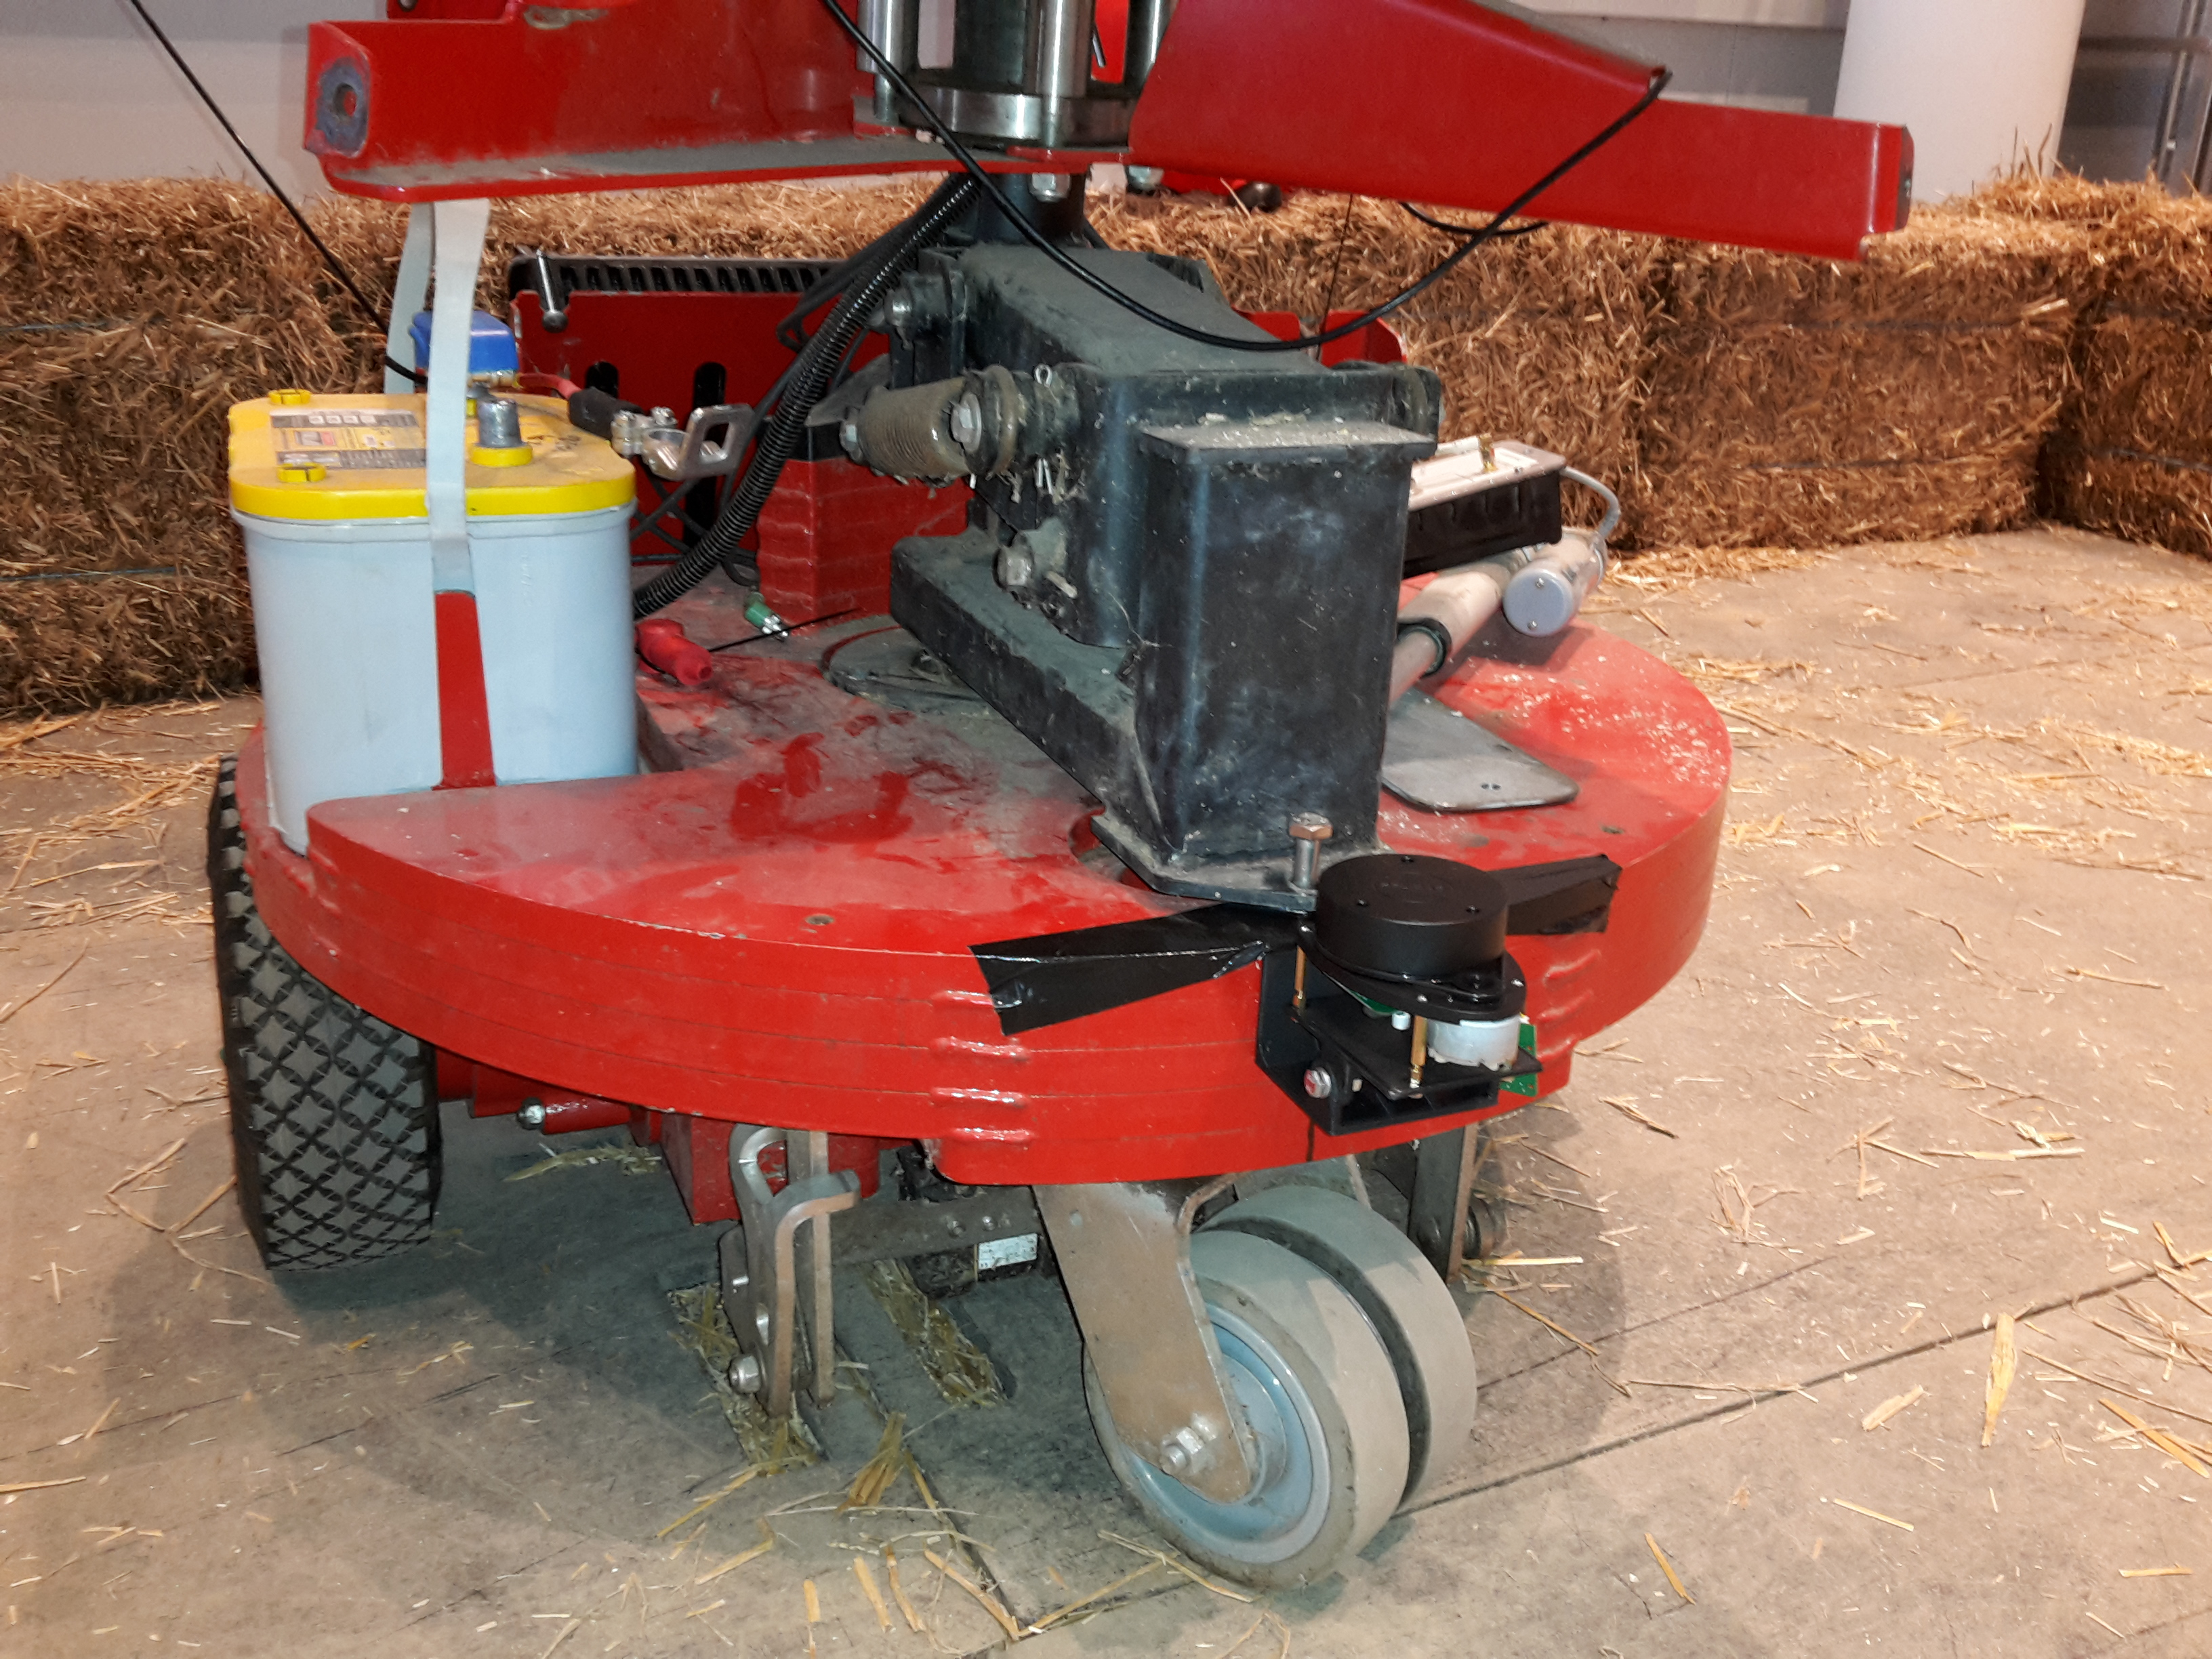
\includegraphics[scale=0.1]{robot_a}
		\caption{The LIDAR sensor and 3D-printed mounting point attached to Robot A}
	\end{figure}
	
	\subsection{Sensors}
	A RPLIDAR A1M8-R6 LIDAR is mounted on the front of the robot. The LIDAR interfaces with the laptop directly over USB. \newline
	
	The A1M8-R6 was chosen due to its excellent support in the ROS ecosystem, allowing for the implementation of a straightfoward navigation stack. 
	
	\subsection{Hardware}
	A 3D-printed mount was created for easy placement and adjustment of the LIDAR. It consists of two parts: the baseplate, which is directly connected to the sensor, and the connector plate, which is taped on the lower platform of the Juno. Both plates are connected through two screws, which form a one degree of freedom joint. This allows the horizontal adjustment of the baseplate, to gain more accurate data from the LIDAR. 
	
	\begin{figure}[h!]
		\centering
		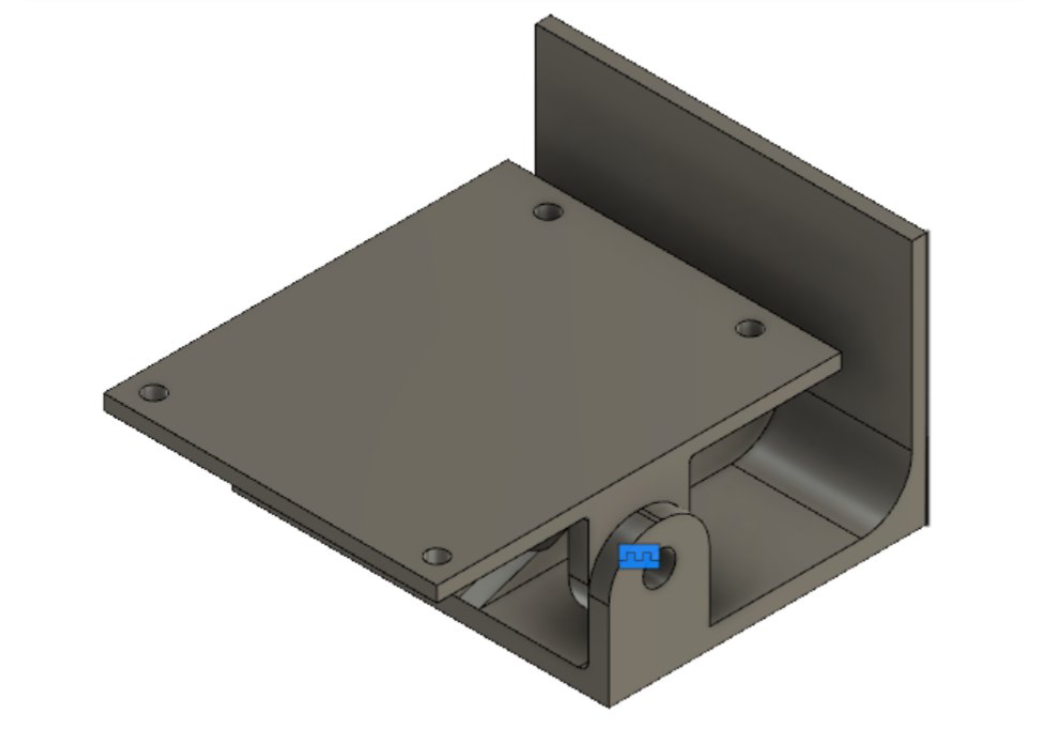
\includegraphics[scale=0.6]{lidar_mount}
		\caption{CAD rendering of LIDAR mount}
	\end{figure}
	
	\subsection{Software}
	The A1M8-R6 LIDAR comes with ROS packages which allow for SLAM mapping without odometry information up to 12 meters. An ideal navigation stack for Robot A would be to use the gmapping ROS package to generate a cost map, allowing for the robot to be steered via the ROS move\_base package. However, due to technical difficulties with move\_base, debugging and testing of this algorithm was not possible. \newline
	
	Attempts at remediating this were unsuccessful within the given time frame.
	
	\pagebreak

	\section{Robot B}
	
	\subsection{Overview}
	Robot B uses ultrasonic sensors mounted via aluminium frame to navigate its environment.
	
	\begin{figure}[h!]
		\centering
		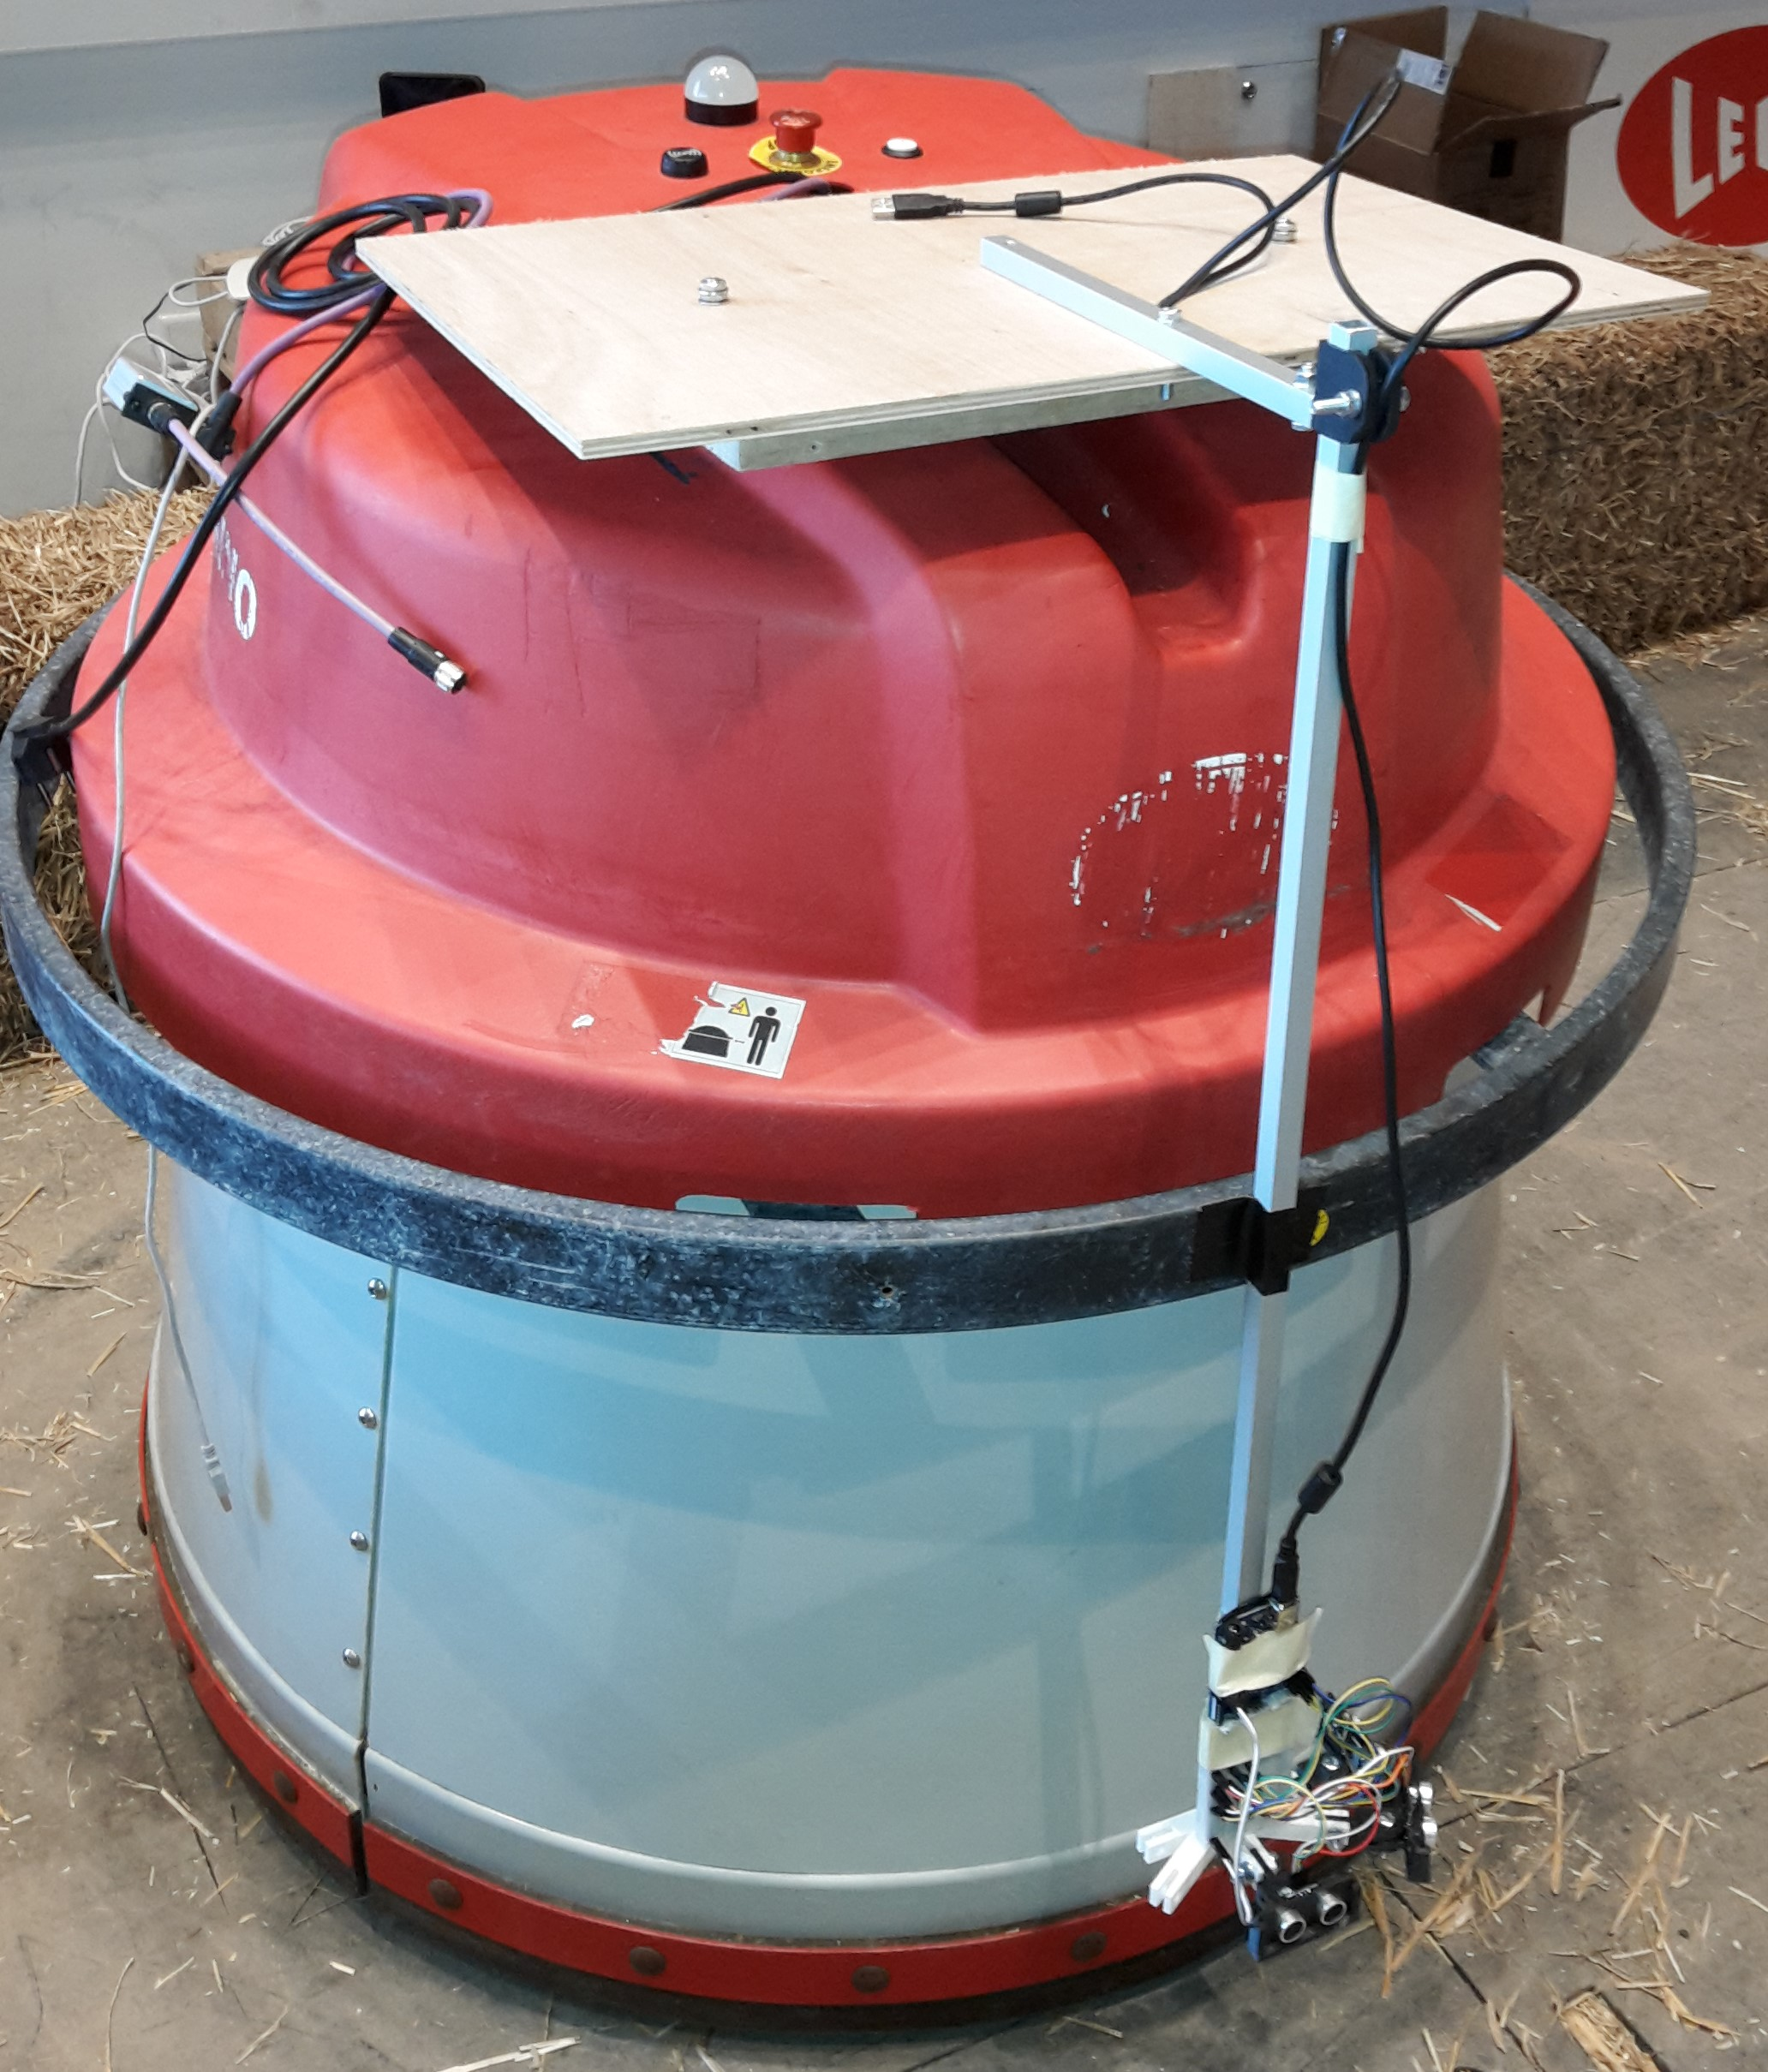
\includegraphics[scale=0.1]{robot_b_full}
		\caption{Robot B with mounting frame, 3D-printed connectors, and ultrasonic sensors}
	\end{figure}
	
	\subsection{Sensors}
	Three HC-SR04 ultrasonic sensors are placed in an array infront of the robot. The sensors interface with the laptop via an Arduino Uno. \newline
	
	A problem faced whilst designing the sensor array was throughput limitations on the Arduino. A single HC-SR04 requires two digital pins for input-output, allowing for a maximum of three sensors per Arduino, as opposed to the originally planned five. \newline
	
	\subsection{Hardware}
	The sensor mounting for Robot B was far more complicated, because it has a complete casing. For this reason, an aluminum frame existing of four edge tubes with 3D-printed connection points extends from the top mounting point to the bottom of the robot, allowing the sensors to attach to a low-enough point to read the walls of the maze.\newline
	
	For accurate sensor data, the ultrasonic sensors should be at the same height as the LIDAR. To implement this, the perpendicular tube is adjustable in height through a clamping mechanism in the connector to the horizontal tube. \newline
	
	To mount all the ultrasonic sensors in a flexible configuration, the mount consists of four different components. Through them, it is possible to adjust the angle and the level of the sensors. \newline
	
	Additionally, they can be easily installed in other configurations or removed for testing reasons.
	
	\begin{figure}[h!]
		\centering
		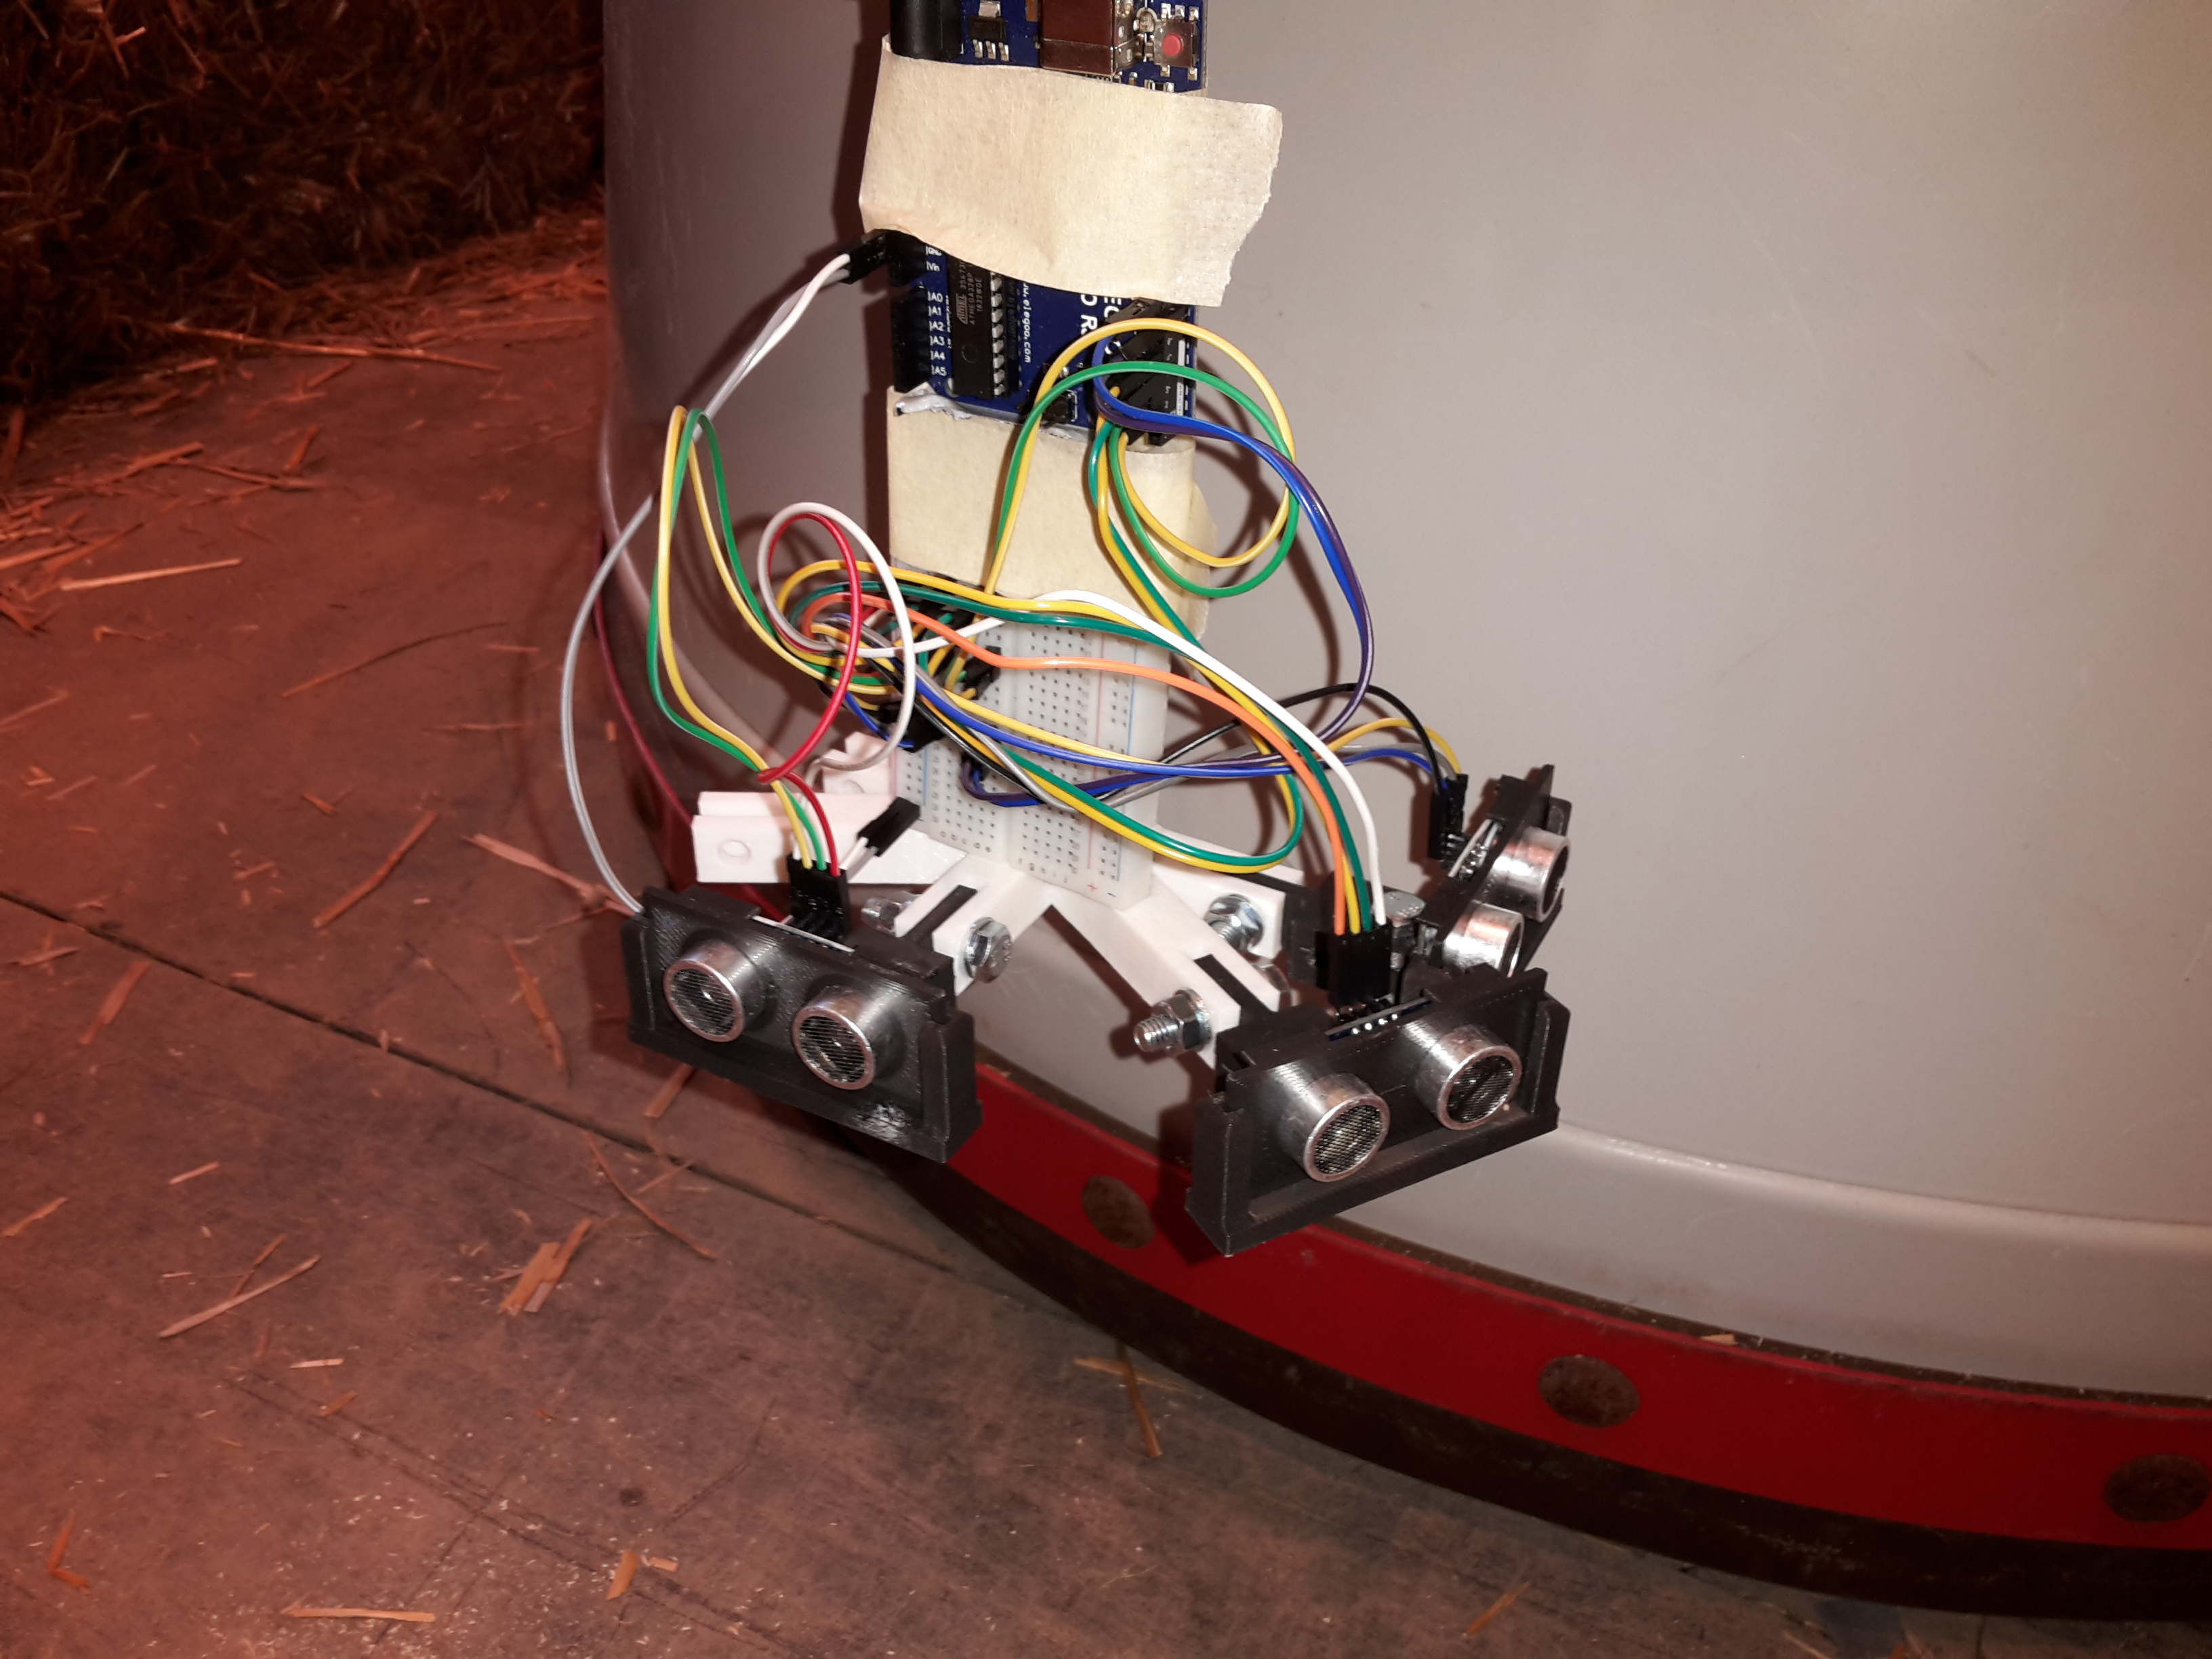
\includegraphics[scale=0.1]{ultrasonic_mount}
		\caption{Robot B with mounting frame, 3D-printed connectors, and ultrasonic sensors}
	\end{figure}
	
	\begin{figure}[h!]
		\centering
		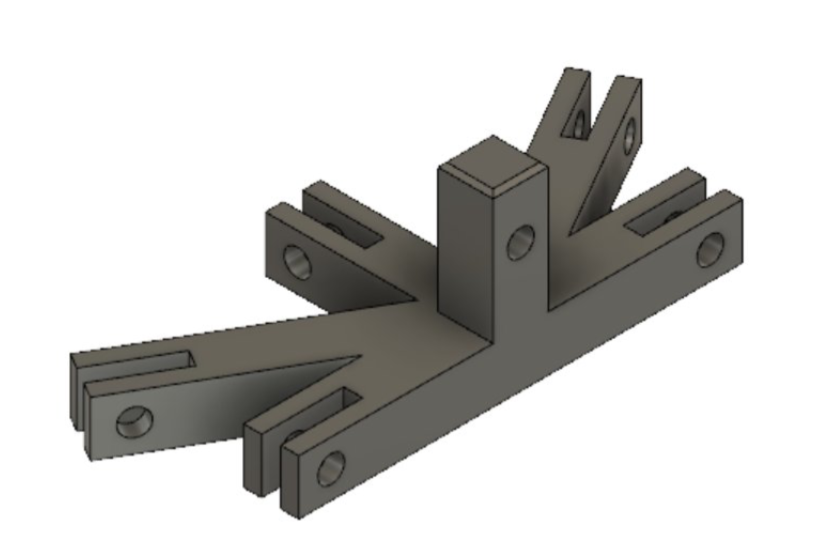
\includegraphics[scale=0.5]{central_mount_empty}
		\caption{Central mount for connection points}
	\end{figure}

	\begin{figure}[h!]
		\centering
		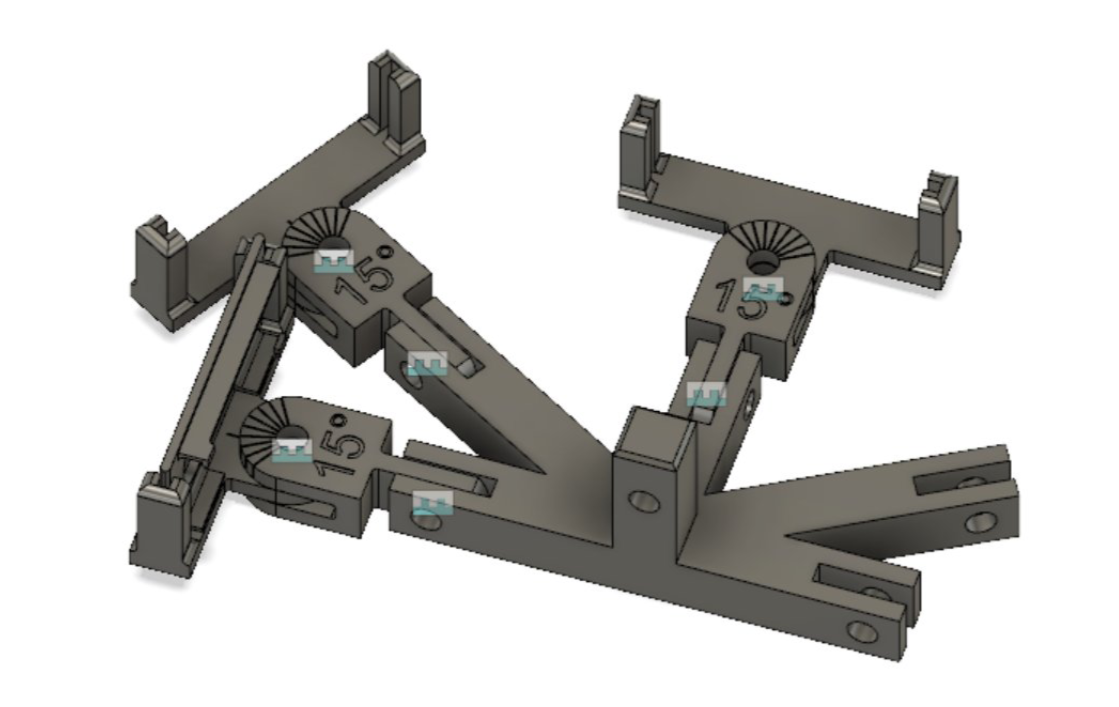
\includegraphics[scale=0.5]{central_mount_conns}
		\caption{Central mount with connections for ultrasonic sensors}
	\end{figure}

	\pagebreak
	
	\subsection{Software}
	The algorithem for Robot B is similar to the case of Robot A. After having received the LIDAR map and its own initial position and orientation from Robot A, Robot B uses a wall following and corner counting algorithem to navigate. The initial position is also used to return to its home base. \newline
	
	This was not realised due to the previous mentioned troubles whilst developing the code for Robot A.
	
\end{document}